\chapter{IO Operations, Interrupts, and Their Impact on Embedded Systems}

\begin{figure}[H]
    \centering
    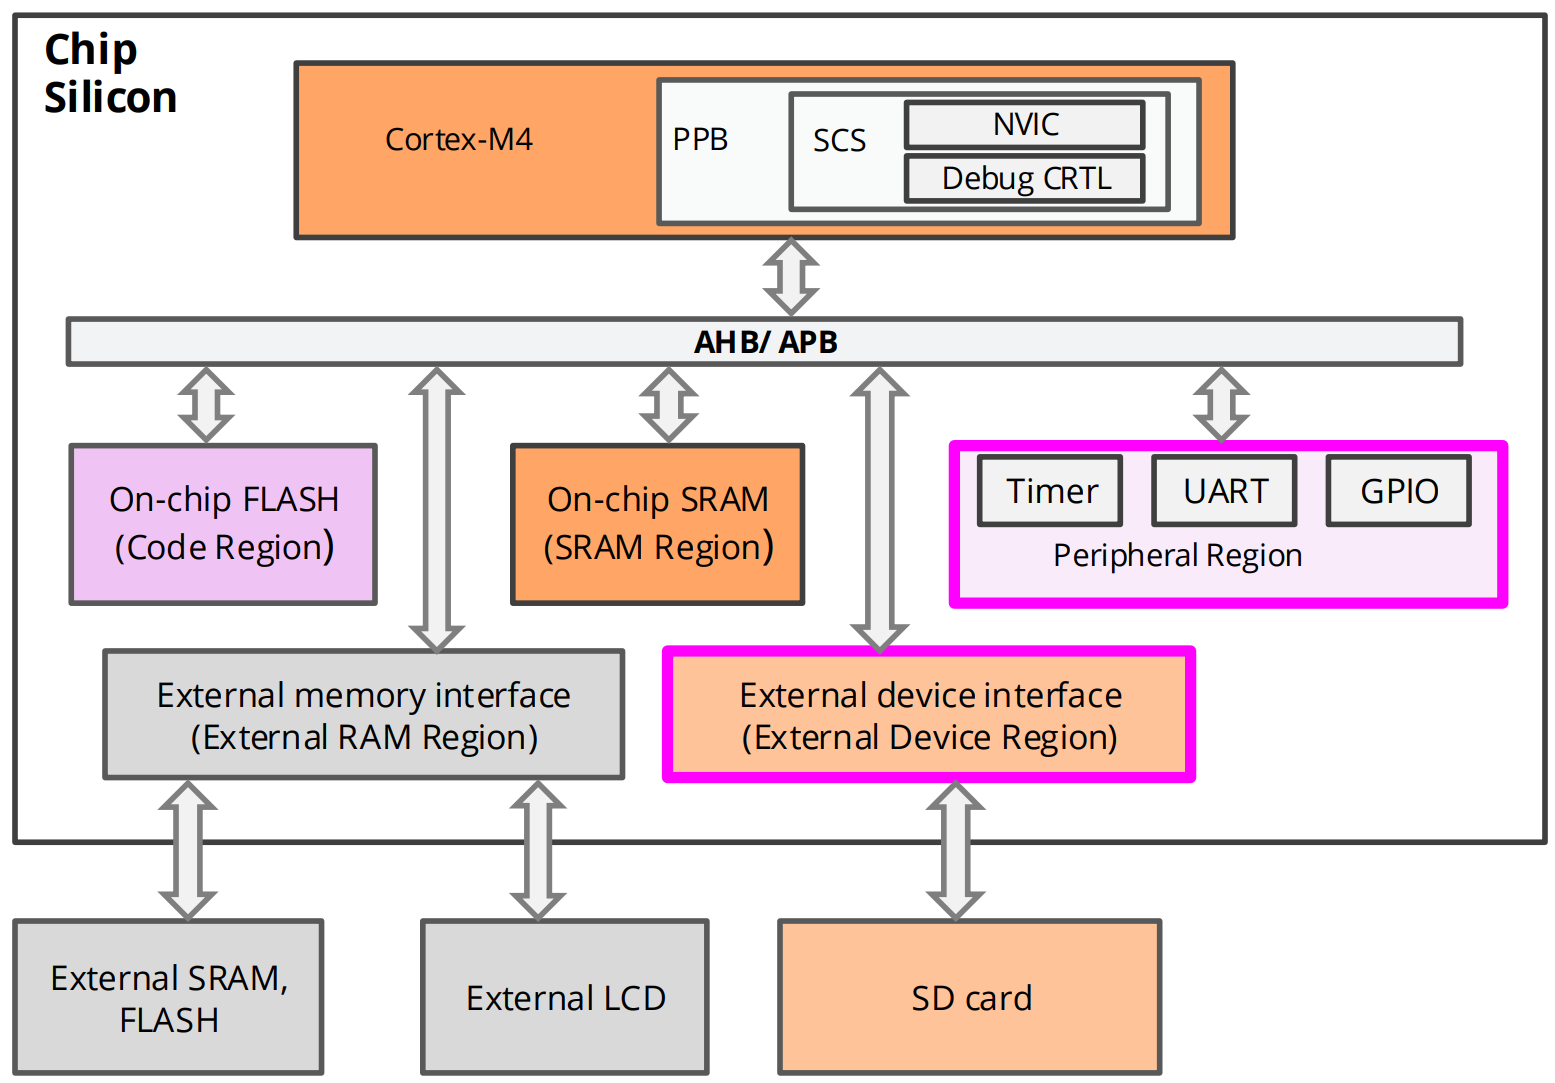
\includegraphics[width=0.8\linewidth]{img/image40.png}
    \caption{Input and Output Devices}
\end{figure}

\section{Current state of Art}
Currently Arm architecture dominates the embedded market. But there is a trend of switching to RISC-V.


\paragraph{}
The benefits is that RISC-V is open-source and more customisable. Because it's open-source this means
it's cheaper to develop with as there are no licensing fees or royalties to pay. ARM is dominant in the
embedded device market but RISC-V is getting more and more use in research and niche markets,
allowing reduced vendor lock-in and greater innovation.

\paragraph{}
\textbf{ARM} processors seem to be more \textbf{power-efficient} for now. \textbf{RISC-V's ecosystem} is growing but it \textbf{is not as
mature and rich as ARM's.}

\newpage
\section{Programming Input and Output}

The CPU talks to the device by reading and writing device registers.

\begin{figure}[H]
    \centering
    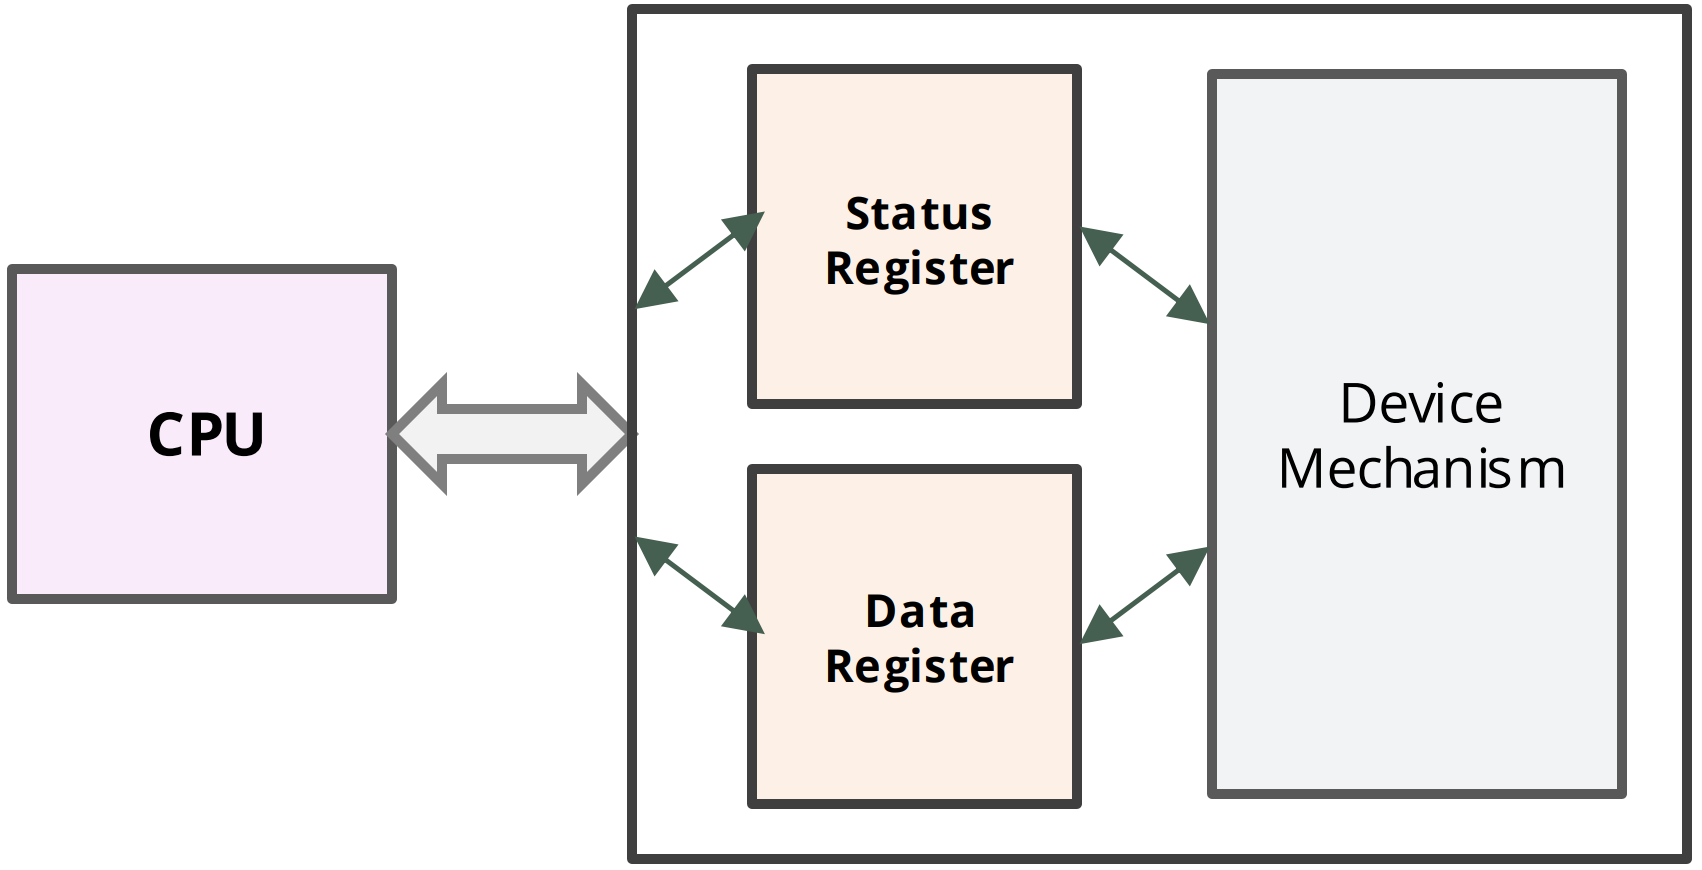
\includegraphics[width=0.6\linewidth]{img/image41.png}
\end{figure}

Devices typically have several registers:

\begin{itemize}
    \item[-] Data registers: hold data values, can be \textbf{readable or writable};
    \item[-] Status registers: provide information about the device's operation, can be \textbf{read-only}
\end{itemize}


\subsection{How to access the registers}

There are two way to access those registers:

\begin{itemize}
    \item[] \textbf{I/O instructions:} special instructions for input (read) and output (write) (in and out in case of Intel x86), requires a separate address space for each I/O device
    \item[] \textbf{Memory-mapped I/O:} the registers are mapped to the memory space of the device, meaning that we will need to manipulate the dedicated registers via normal memory read and write to communicate with devices. Very simple way.
\end{itemize}

We will use memory-mapped I/O throughout the course.


\subsection*{Example: Memory-mapped I/O on ARM}

Define location for device and provide Read/Write code:

\begin{lstlisting}[language=c++]
    DEV1 EQU 0x1000
    LDR r1,#DEV1 ; set up device addres
    LDR r0,[r1] ; read DEV1
    LDR r0,#8 ; set up value to write
    STR r0,[r1] ; write value to device
\end{lstlisting}


\subsection*{Example: write I/O in C}

We can use pointers to manipulate the addresses of I/O devices

\begin{lstlisting}[language=c]
    int read(char *location) {
        return *location;
    }
    void write(char *location, char newval) {
        (*location) = newval;
    }

\end{lstlisting}

To read a device register we can write:

\begin{lstlisting}[language=c]
    #define DEV1 0x1000
    ...
    dev_status = read(DEV1); /* read device register */
\end{lstlisting}

To write to the status register, we can use the following code:

\begin{lstlisting}[language=c]
    write(DEV1,8); /* write 8 to device register */
\end{lstlisting}


\section{Busy-Wait I/O}

Devices are typically slower than the CPU, so they may require many cycles to complete an operation.

The Busy-Wait, a.k.a. polling,  is a technique in which the CPU keeps asking the I/O
device if it has finished the operation by checking its status register.

\subsubsection{Example: Busy-Wait I/O}

We need to write a sequence of characters to an output device. The device has two registers, one for the
character to be written and a status register.

The status register's value is 1 when the device is busy writing and 0 when the write has completed.


\begin{lstlisting}[language=C]

    #define OUT_CHAR 0x1000 /* output device character register */
    #define OUT_STATUS 0x1001 /* output device status register */
    ...
    char *mystring = "Hello, world." /* string to write */
    char *current_char; /* pointer to the current position in string */
    current_char = mystring; /* point to the head of string */
    while (*current_char != '\0') { /* until null character */
        write(OUT_CHAR,*current_char); /* send character to device */
        while (read(OUT_STATUS) != 0); /* keep checking status */
        current_char++; /* update character pointer */
    }   
\end{lstlisting}

As shown in the example, we write one character each then check if the device has finished writing to
send the next one.

\paragraph{}
When a new character has been read: the input device sets its status register to 1, we must set it back to 0 so that the device is ready to read another character 

\paragraph{}To start writing: first set the output status register to 1, then wait for it to return to 0.

\subsubsection{Example 2: Busy-Wait I/O}
The following example showcases a simple application involving an input device and an output device
connected to the same CPU.

\begin{lstlisting}[language=C]

    #define IN_DATA 0x1000
    #define IN_STATUS 0x1001
    #define OUT_DATA 0x1100
    #define OUT_STATUS 0x1101
    ...
    while (TRUE) { /* perform operation forever */
    /* read a character into achar */
    
    while (read(IN_STATUS) == 0); /* wait until ready */
        achar = (char)read(IN_DATA); /* read the character */
        write(OUT_DATA,achar); /* write achar */
        write(OUT_STATUS,1); /* turn on device */
        while (read(OUT_STATUS) != 0); /* wait until done */
    }   
\end{lstlisting}

The code is supposed to get input from a keyboard and then show it onto an LCD display:

\begin{itemize}
    \item[-] It keeps waiting until the input device's status is set to ready, indicating a new character
    \item[-] It reads the new character and stores it in memory
    \item[-] It writes the new character in the data register of the output device
    \item[-] It keeps waiting until the output device's status is set to ready, indicating a new character can be written
\end{itemize}

\subsection{Cons of using Busy-Wait I/O}

The bad side of busy-wait is that we waste too many CPU cycles (extremely inefficient), which is not
ideal when there are many I/O devices connected.

The most effective way is not to check all the time, but to be notified automatically. This is why the
interrupt mechanism is used, allowing devices to signal the CPU and force execution of a
particular piece of code (interrupt handler).


\section{Interrupt: How it Works}

\begin{figure}[H]
    \centering
    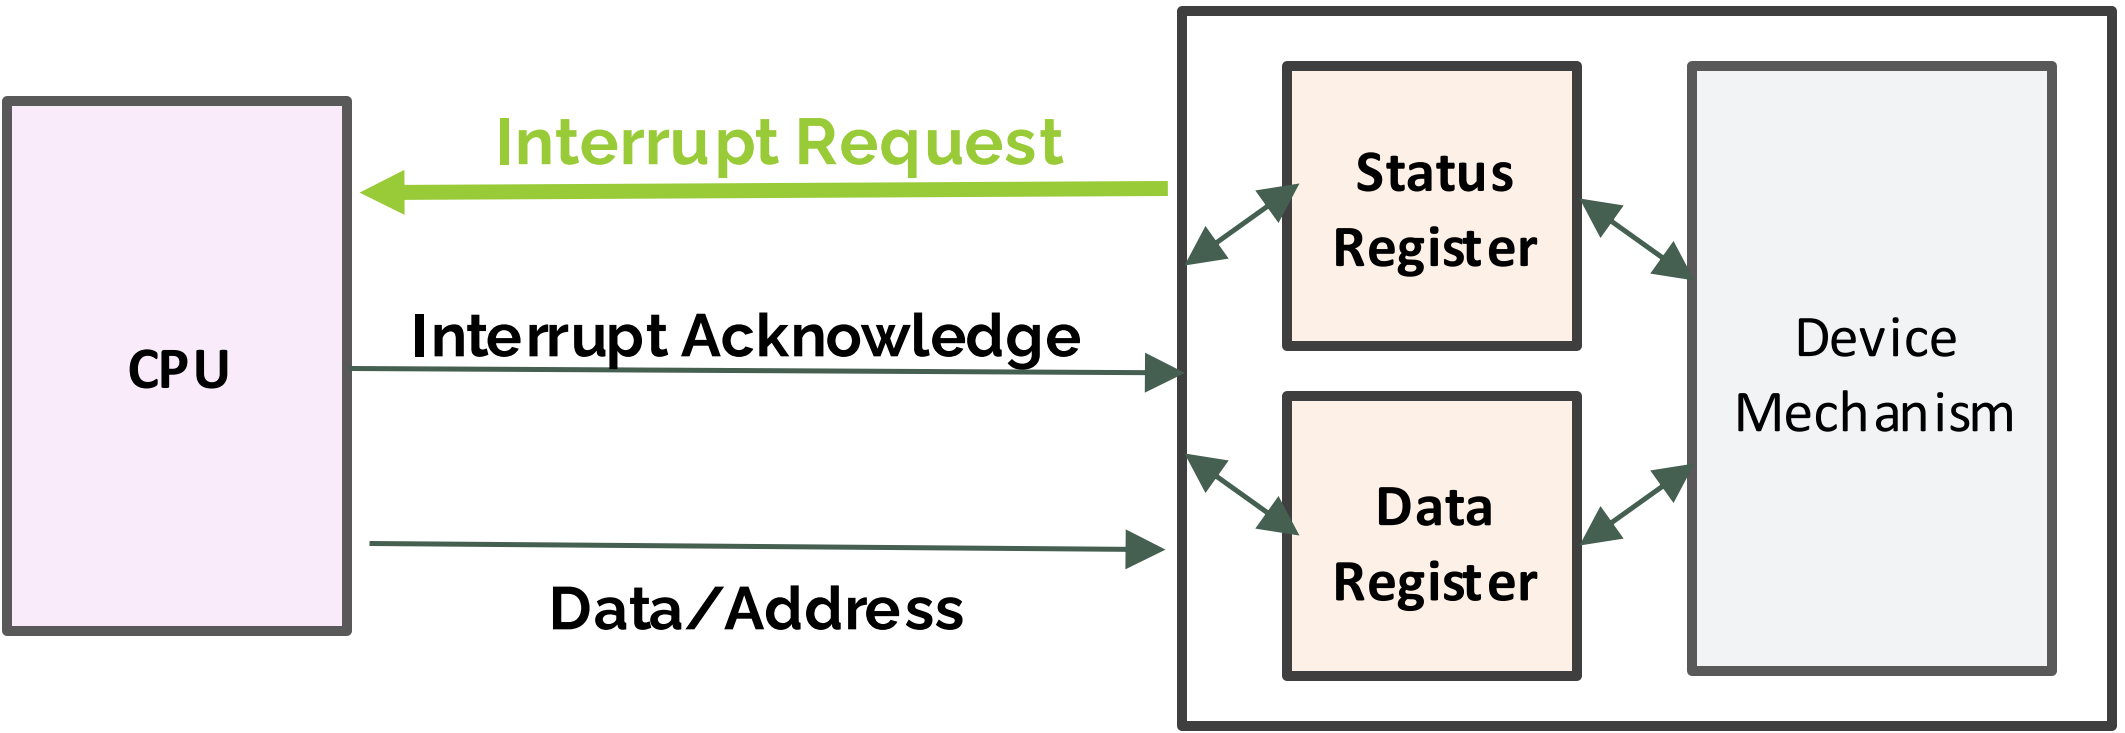
\includegraphics[width=0.65\linewidth]{img/image43.png}
\end{figure}

An interrupt works with the following steps (high-level overview):

\begin{enumerate}
    \item the I/O device decides when to interrupt, like when its status register goes into the ready state
    \item the I/O device wants service from the CPU, so it sends an interrupt request signal
    \item the CPU checks the interrupt request (IRQ) line at every instruction
    \item the CPU is ready to handle the I/O device's request, so it sends an interrupt acknowledge signal
    \item the CPU saves the current value of the program counter
    \item the CPU then changes the program counter to point to the device's interrupt handler
    \item the starting addresses of the interrupt handlers are stored in a table called Interrupt Vector Table/Interrupt Handler Table stored in the CPU's memory
    \item after execution, the interrupt handler executes a special instruction called IRET or RETI to signal it finished execution
    \item the CPU then switches back to the previous program counter to resume its normal execution
\end{enumerate}

\subsection{Priorities and Vectors}

As most systems have more than I/O device, multiple devices can interrupt even at the same time. In this
case, the interrupts are ran in order of priority via a \textbf{Programmable Interrupt Controller} (\textbf{PIC}).

\begin{figure}[H]
    \centering
    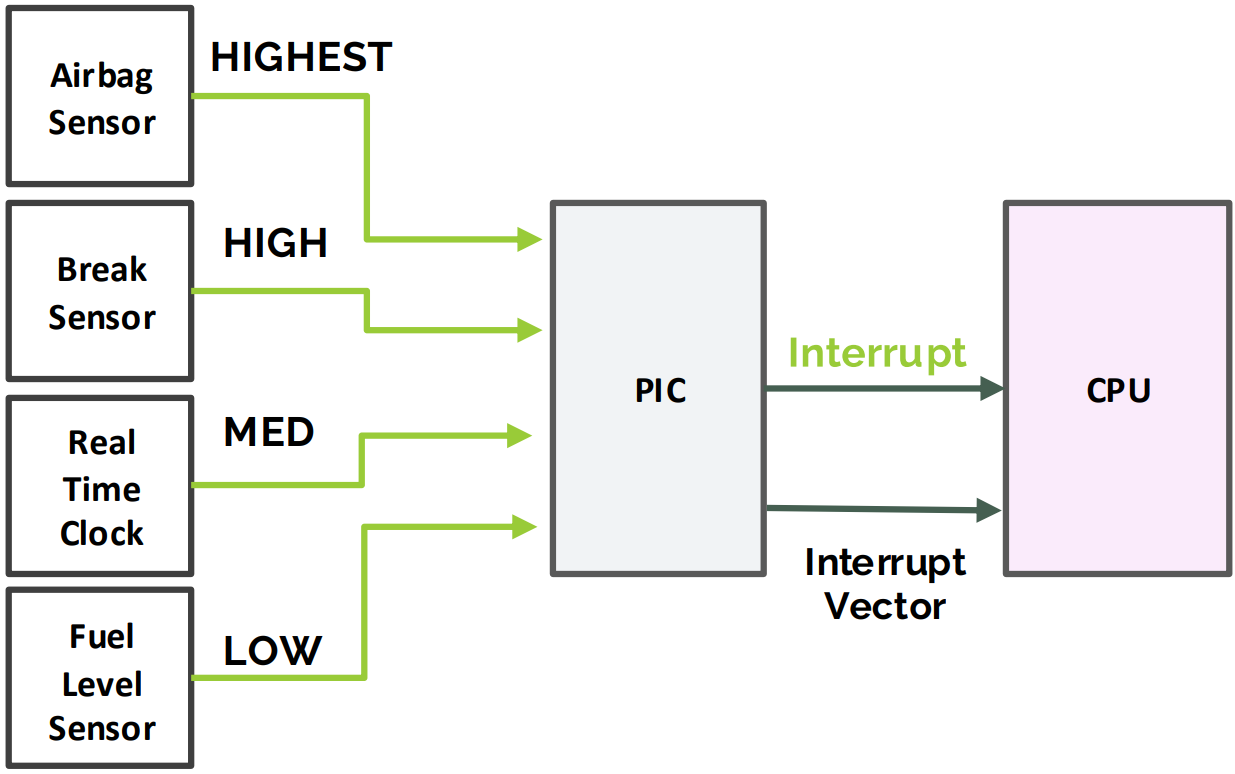
\includegraphics[width=0.65\linewidth]{img/image46.png}
\end{figure}

In the ARM architecture it is called the \textbf{Nested Vector Interrupt Controller} (\textbf{NVIC}). Also it is the interrupt device that specifies its interrupt handler (the index in the Interrupt Vector Table).

\begin{figure}[H]
    \centering
    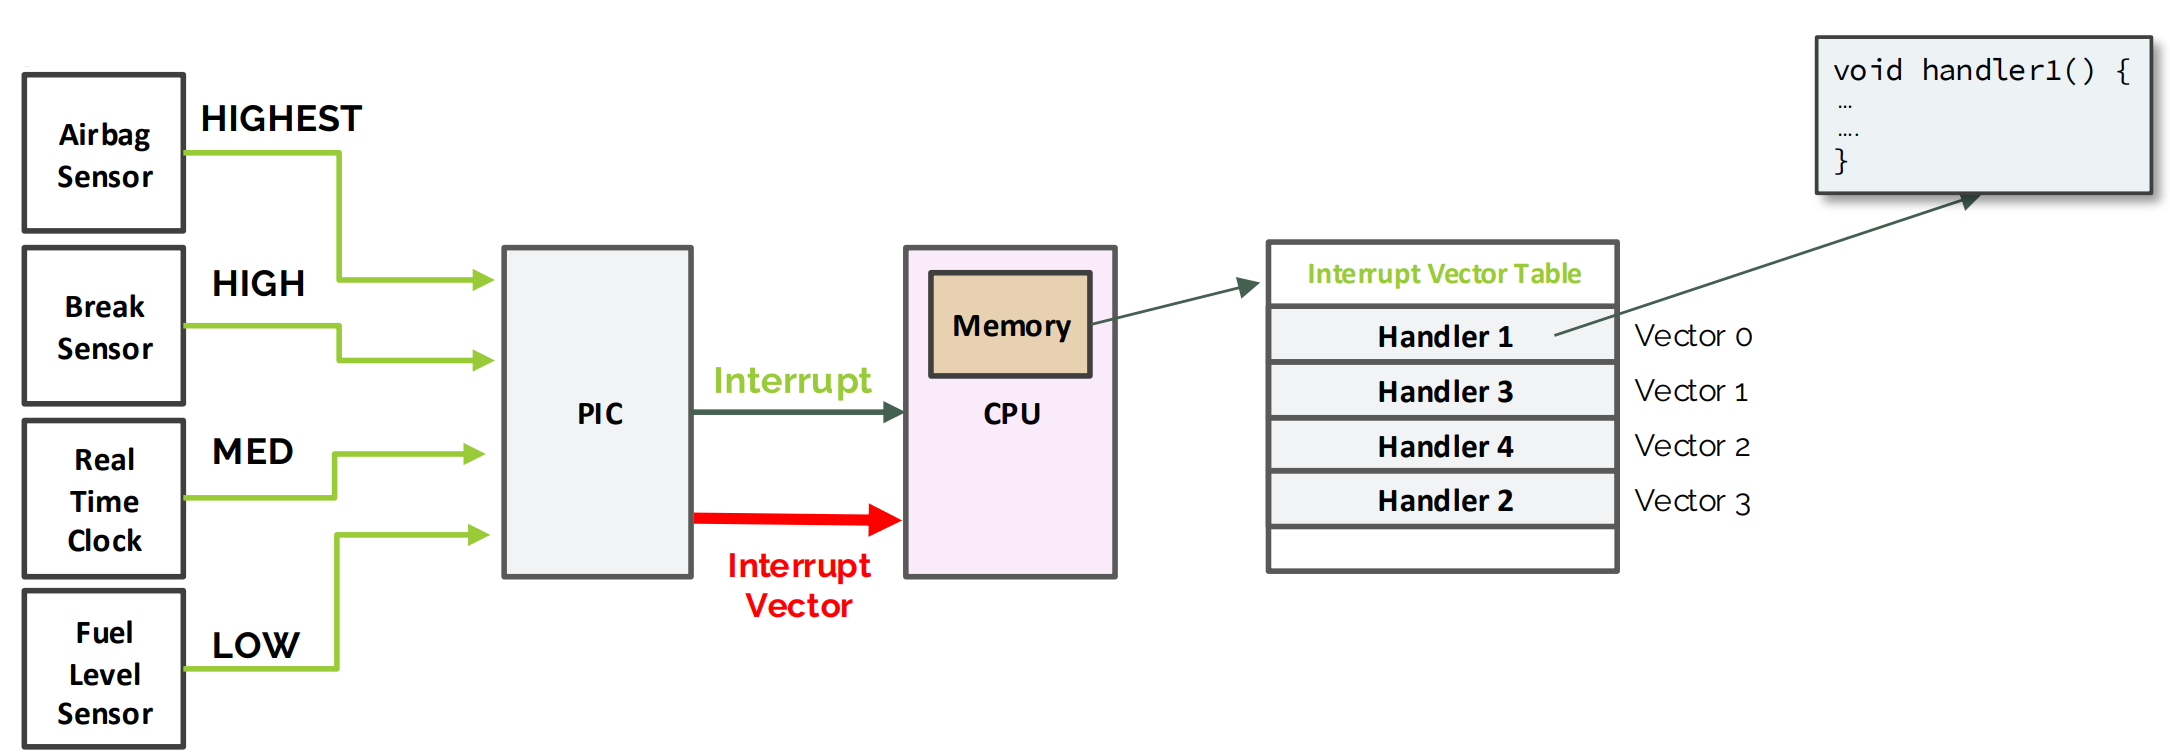
\includegraphics[width=1\linewidth]{img/image44.png}
\end{figure}

\begin{figure}[H]
    \centering
    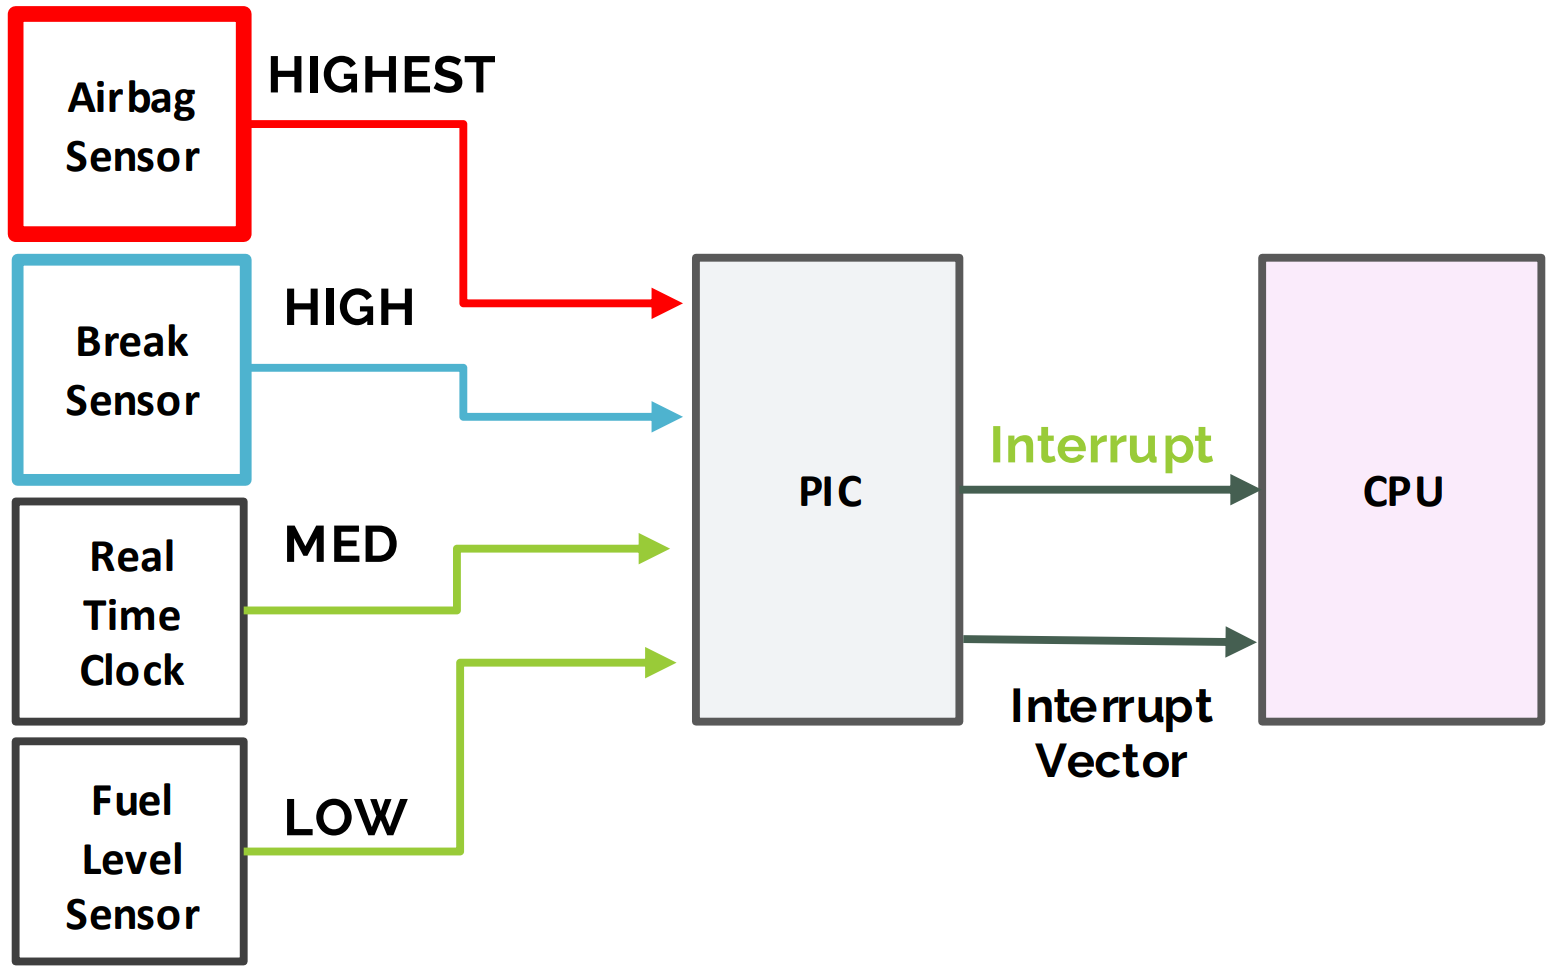
\includegraphics[width=0.65\linewidth]{img/image47.png}
\end{figure}


\paragraph{}
The interrupt devices are connected to the PIC, which tells them if their interrupt handlers are being
executed or are in line through interrupt acknowledge lines. If they are in line, they will also know their
own number of priority.

\begin{figure}[H]
    \centering
    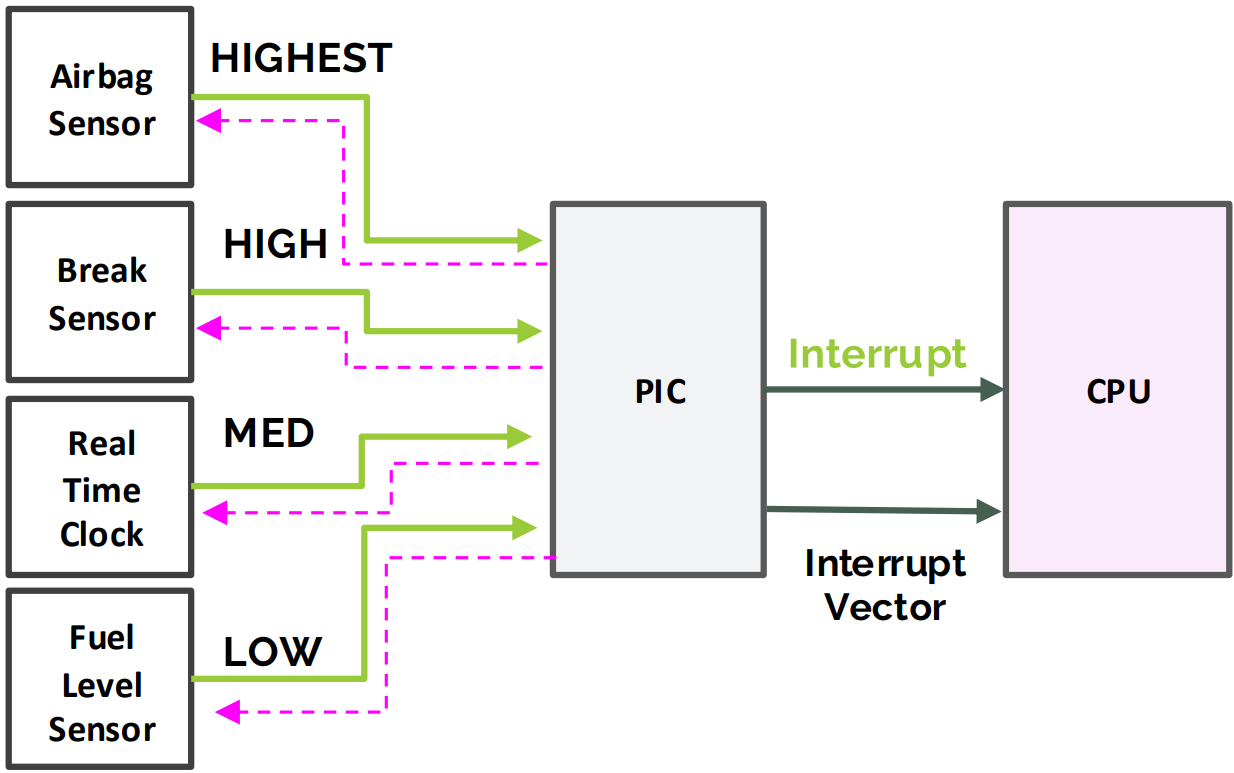
\includegraphics[width=0.65\linewidth]{img/image48.png}
\end{figure}

Nested interrupts must be prevented (ISR being ran while another ISR is being ran already).

\paragraph{NOTE: } Interrupt handler = ISR = Interrupt Service Routine


\begin{figure}[H]
    \centering
    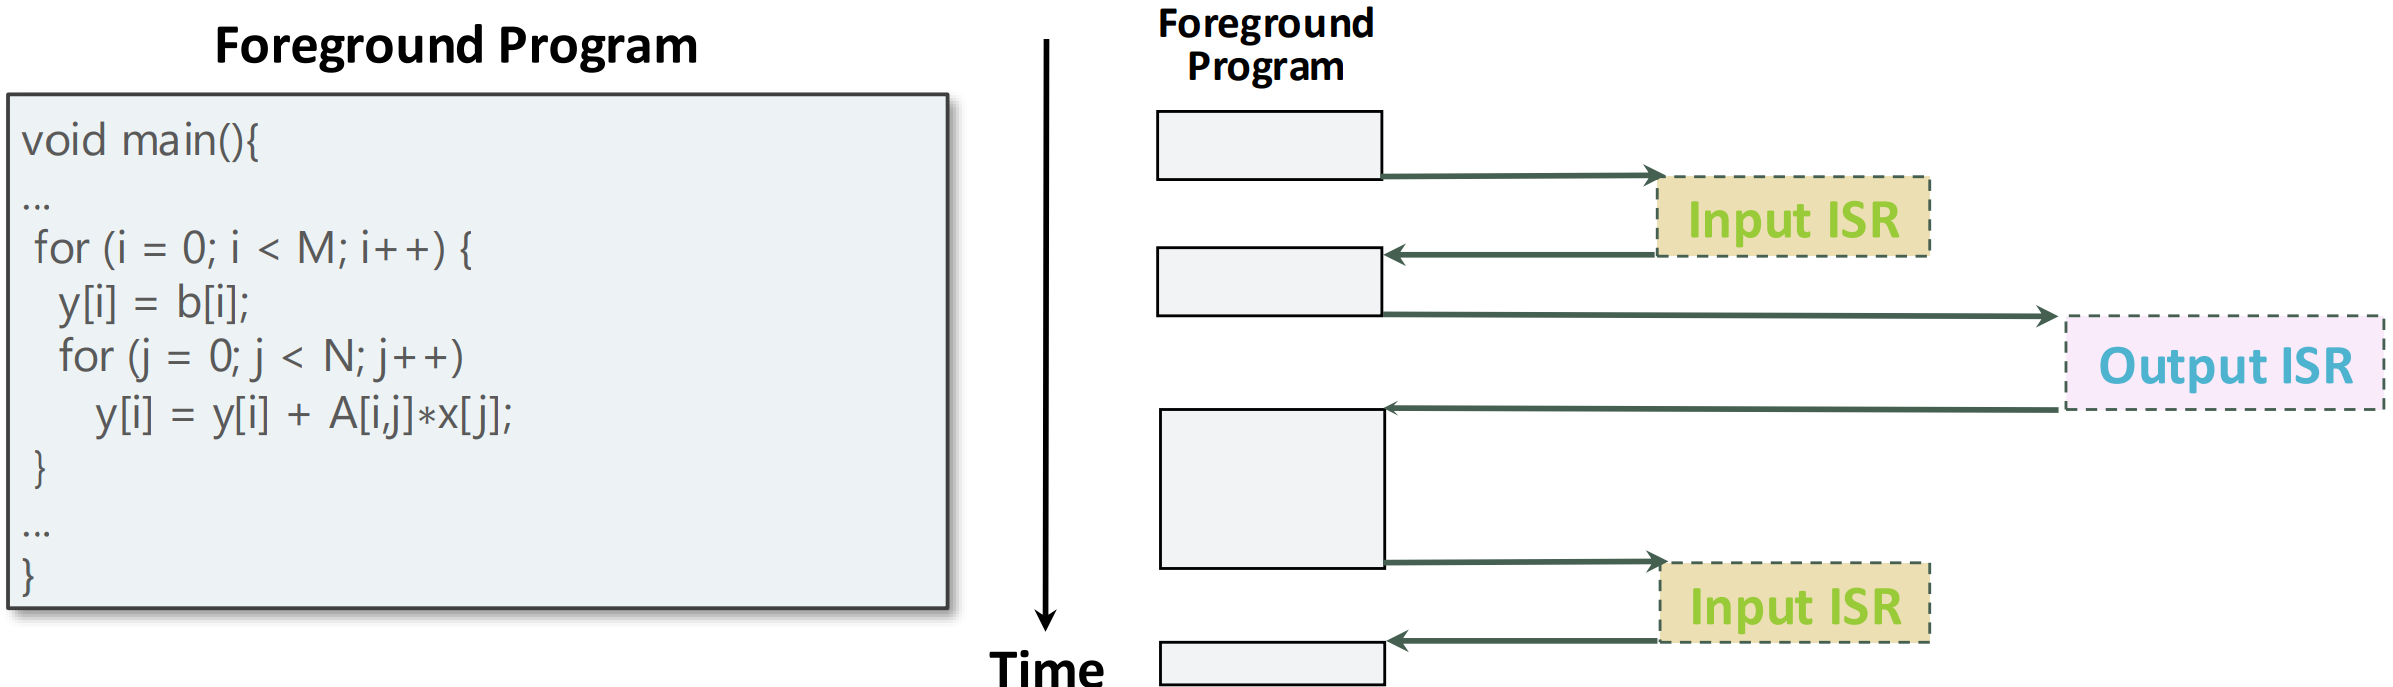
\includegraphics[width=0.9\linewidth]{img/image42.png}
\end{figure}


\section{Interrupt Masking}

Interrupt masking is a technique used to control and prioritize interrupt handling. It is typically used
to ensure that high-priority interrupts are handled promptly, especially in real-time and safety-critical
systems where specific interrupts must be handled immediately to meet timing or safety requirements.

\paragraph{"Masking"} means temporarily disabling an interrupt. This means that as soon as the CPU
acknowledges a higher priority interrupt, it immediately pauses the current ISR, executes the higher
priority interrupt's ISR before resuming the previous one.

The \textbf{PIC} is used to facilitate interrupt masking, via registers or configuration settings to enable or disable
specific interrupt sources.


\section{Non-Maskable Interrupt}

Non-maskable interrupt (NMI) is an interrupt that cannot be masked so it will be executed 100% instantly
without getting turned off. It is usually reserved for interrupts caused by power failures to save critical
state in nonvolatile memory, turn off I/O devices...

NMIs are device specific.



\section{Interrupt vs Exceptions}

While \textbf{both do the same thing} (interrupt the current flow of the program), interrupt is meant when it's done
by a \textbf{hardware device}, while an exception is done by the \textbf{software}.

\subsection{Example \#1: interrupt}


The following example showcases the same program from the previous example, now using interrupts:

\begin{lstlisting}[language=c]

    /* get a character and put in global (called when IN_STATUS is 1) */
     
    void input_handler() {
        achar = read(IN_DATA); /* get character */
        gotchar = TRUE; /* signal to main program */
        write(IN_STATUS,0); /* reset status to initiate next transfer */
    }
    
    /* react to character being sent (called when OUT_STATUS is 0) */
    void output_handler() {
        /* don't have to do anything */
    }
\end{lstlisting}

The \verb|input_handler| function does the following:

\begin{itemize}
    \item[-] stores the new character, taken from the input device's data register, into achar
    \item[-] turns gotchar to true to signal to the main program that there's a new character
    \item[-] resets the input device's status register to 0, ready state
\end{itemize}


All input device operations are done in the interrupt handler.


\subsubsection{Mainprogram:}

\begin{lstlisting}[language=c]

    main() {
        while (TRUE) { /* read then write forever */
            if (gotchar){ /* write a character */
                write(OUT_DATA,achar); /* put character in device */
                write(OUT_STATUS,1); /* set status to initiate write */
                gotchar = FALSE; /* reset flag */
            }
        }
    }
\end{lstlisting}

\begin{enumerate}
    \item The gotchar variable is checked if true
    \item Once it is, the character is written in the output device's data register and the output device's status register is set to 1, signaling it to initiate write
    \item Then resets the gotchar variable to false as it waits for a new character
\end{enumerate}

A few issues in this example:

\begin{itemize}
    \item[] output device is not waited for when it finishes writing
    \item[] character can be overwritten before it is written in the output device's data register
\end{itemize}

\textit{This example is used to just show off how interrupts work.}


\subsection{Example \#2: Interrupt}

The following example showcases the previous program but more sophisticated and improved thanks to
the use of a \textbf{wraparound/circular buffer} (data structure) to hold the new characters, which also fixes the
issues of the previous example.


\begin{figure}[H]
    \centering
    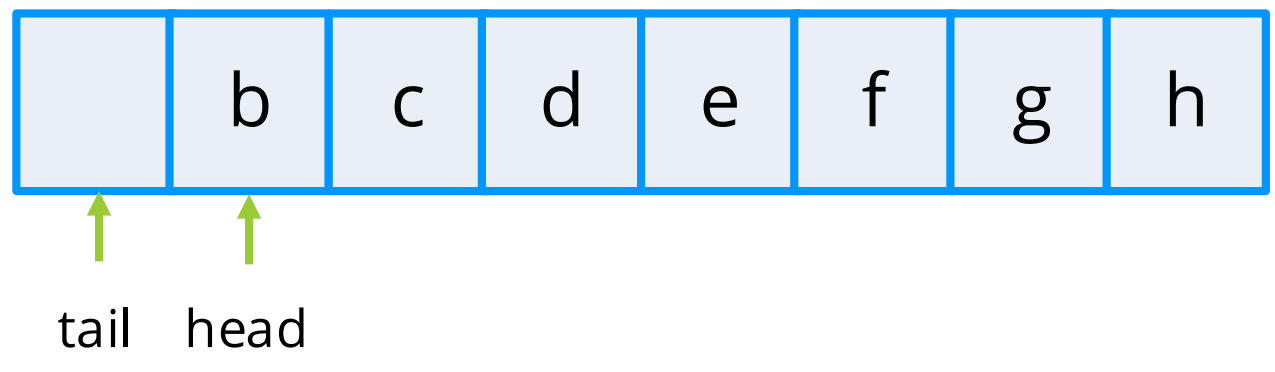
\includegraphics[width=0.6\linewidth]{img/image45.png}
\end{figure}

\subsubsection{Here's an implementation of the circular buffer:}

\begin{lstlisting}

    #define BUF_SIZE 8
    char io_buf[BUF_SIZE]; /* character buffer */
    int buf_head = 0, buf_tail = 0; /* current position in buffer */
    int error = 0; /* set to 1 if buffer ever overflows */
    
    int empty_buffer() { /* returns TRUE if buffer is empty */
        return buf_head == buf_tail;
    }
    
    int full_buffer() { /* returns TRUE if buffer is full */
        return (buf_tail+1) % BUF_SIZE == buf_head ;
    }
    
    int nchars() { /* returns the number of characters in the buffer */
        if (buf_head >= buf_tail)
            return buf_head - buf_tail;
        else
            return BUF_SIZE - buf_tail - buf_head;
    }
    
    void add_char(char achar) { /* add a character to the buffer head */
        io_buf[buf_tail++] = achar;
        /* check pointer */
        if (buf_tail == BUF_SIZE)
        buf_tail = 0;
    }
    char remove_char() { /* take a character from the buffer head */
        char achar;
        achar = io_buf[buf_head++];
        /* check pointer */
        if (buf_head == BUF_SIZE)
            buf_head = 0;
        return achar;
    }
\end{lstlisting}

Here are the new input/output handlers, making use of the circular buffer:

\begin{lstlisting}

    #define IN_DATA 0x1000
    #define IN_STATUS 0x1001
    
    /* get a character (called when IN_STATUS is 1) */
    void input_handler() {
        char achar;
        
        if (full_buffer()) /* error */
            error = 1;
        else { /* read the character and update pointer */
            achar = read(IN_DATA); /* read character */
            add_char(achar); /* add to queue */
        }    
        write(IN_STATUS,0); /* set status register back to 0 */
        
        /* if buffer was empty, start a new output transaction */
        if (nchars() == 1) { /* buffer had been empty until this interrupt */
            write(OUT_DATA,remove_char()); /* send character */
            write(OUT_STATUS,1); /* turn device on */
        }
    }
\end{lstlisting}

\begin{lstlisting}

    #define OUT_DATA 0x1100
    #define OUT_STATUS 0x1101
    
    /* react to character being sent (called when OUT_STATUS is 0) */
    void output_handler() {
        if (!empty_buffer()) { /* start a new character */
            write(OUT_DATA,remove_char());/* send character */
            write(OUT_STATUS,1); /* turn device on */
        }
    }
\end{lstlisting}

The input handler writes the data to the output device when the buffer is empty.

When the buffer is not empty, the output handler keeps writing data to the output device while emptying
the buffer.

\subsection{Cons of Interrupts}

\begin{itemize}
    \item Interrupts increase the program's complexity
    \item Finding bugs is difficult because interrupts are triggered by hardware devices
    \item Concurrency with interrupt handlers can cause bugs if they don't save/restore CPU registers that they modify during executions, causing variables in the foreground program to change mysteriously
\end{itemize}

\section{Overhead of Interrupts}

An interrupt causes a change in the program counter, which incurs a branch penalty: the pipeline of
instructions gets invalidated. So if interrupts occur frequently there will be a noticeable overhead.


If the interrupt automatically stores CPU registers, it requires extra cycles.


Also the acknowledgements, priorities, and the obtaining the index in the table from the device all require
extra cycles.

\paragraph{}
All around interrupts add overhead and latency to the device.
Real-time, or time-critical applications require great knowledge of interrupt and its mechanisms as to
minimise overhead.

\begin{figure}[H]
    \centering
    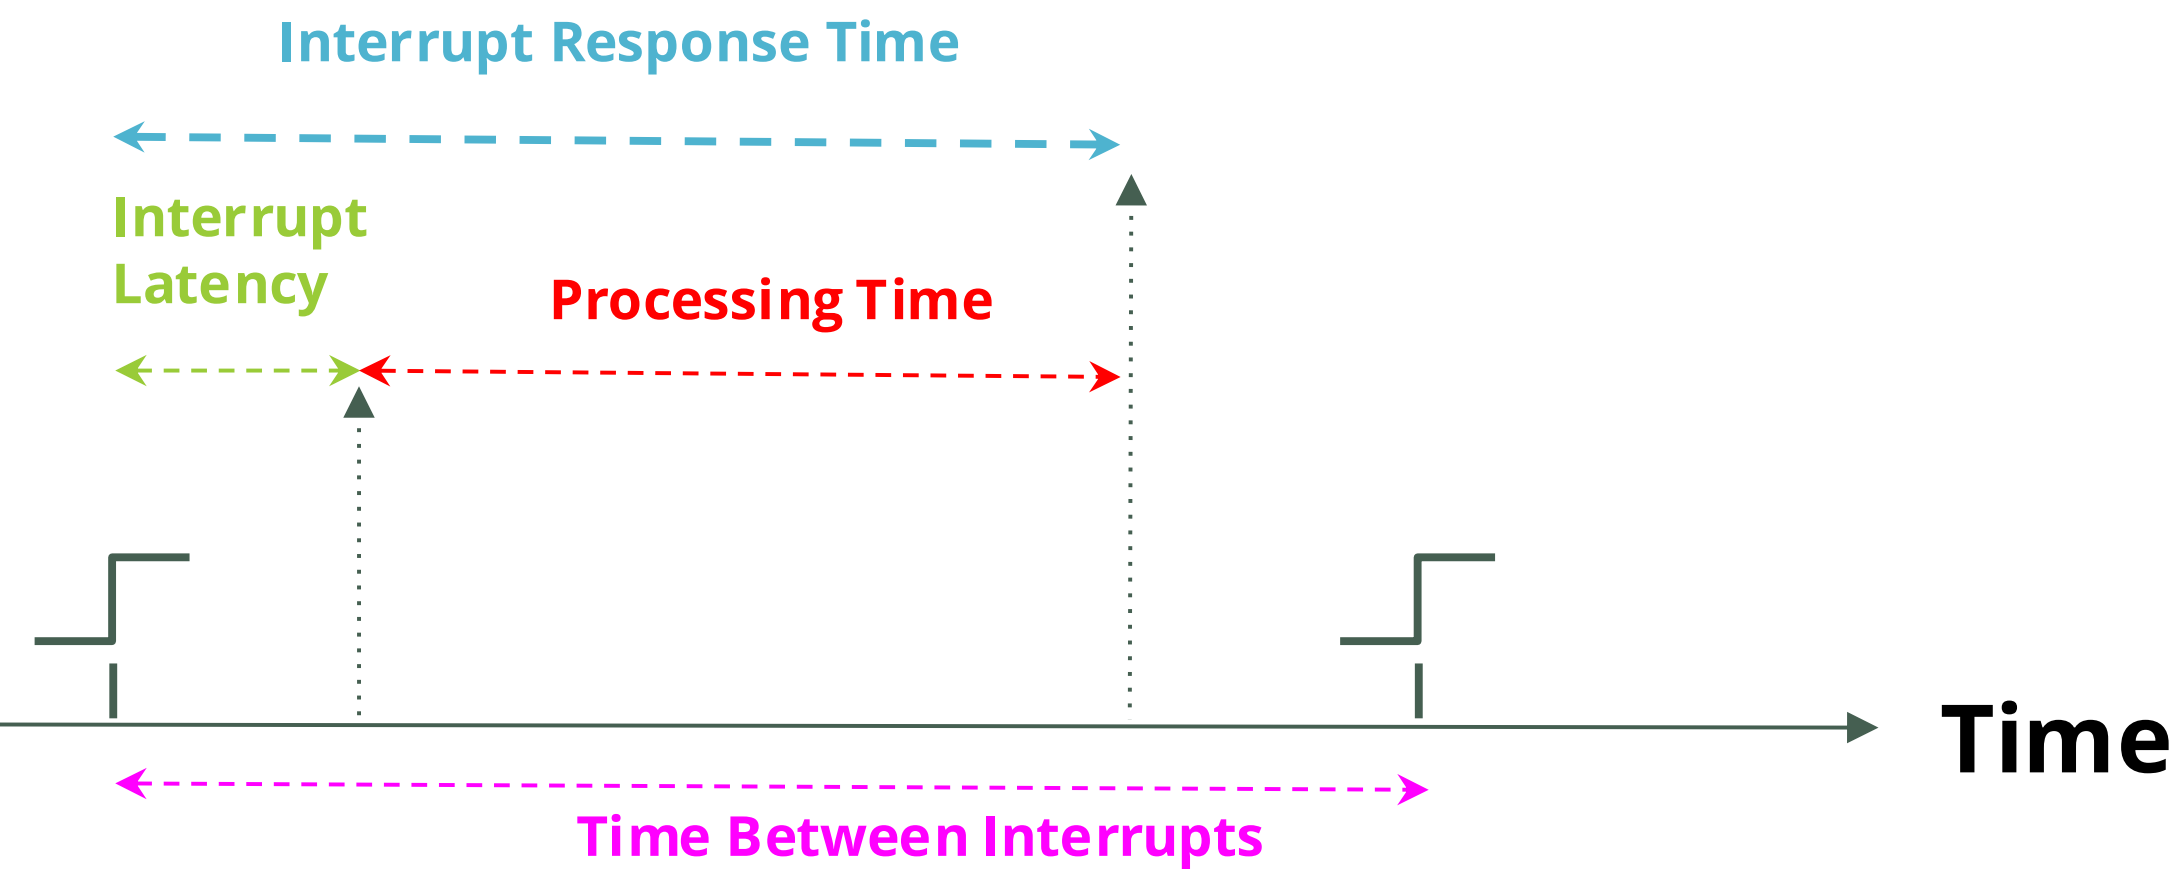
\includegraphics[width=0.85\linewidth]{img/image49.png}
\end{figure}

\section{Co-processors}

They are processors attached to the CPU that implement some instructions, mostly maths instructions. The
most common co-processor adds \textbf{floating-point arithmetic capabilities}.

A co-processor has its own registers and hardware. The co-processor is ordered by the CPU to activate, receive the instruction and execute it when it receives
a co-processor instruction via certain opcodes reserved in the instruction set.


The CPU can either:

\begin{itemize}
    \item suspend execution to wait for the co-processor to finish
    \item continue executing instructions (super-scalar approach)
\end{itemize}